\documentclass[a4paper]{report}
%\documentclass[a5paper,12pt,landscape]{report}

%\usepackage[margin=1cm]{geometry}

\usepackage[T1]{fontenc}
\usepackage[english]{babel}
%\usepackage[utf8]{inputenc}

\usepackage{tikz}
\usetikzlibrary{calc}
\usetikzlibrary{arrows, backgrounds}

%\usepackage{amsfonts}
%\usepackage{amsmath}
%\usepackage{amsthm}
\usepackage{bm}

\usepackage{graphicx}
\graphicspath{{../fig/}}
\usepackage{subfig}

\usepackage{caption}
\captionsetup{font=footnotesize}

\newcommand*\V[1]{\bm{#1}}
\newcommand{\E}{\V{E}}
\newcommand{\B}{\V{B}}
\renewcommand*{\v}{\V{v}}
\newcommand{\x}{\V{x}}
\newcommand{\dt}{\Delta t}
\newcommand{\dx}{\Delta x}

\title{Simulation of plasma with \texttt{cpic} using OmpSs}
\author{Rodrigo Arias Mallo}
\date{\today}

\begin{document}

\maketitle
\tableofcontents

\chapter{Introduction}

It may be surprising to find out that the most common state of matter is plasma 
when we look at the universe. A plasma is a gas in which at least one electron 
of the atom is separated, so it remains positively charged (ionized) 
\cite{chen}.  Usually this happens in the vacuum

\chapter{Plasma simulation}


\subsection{The particle in cell method (PIC)}

%TODO: Show the main equation
Solving the Vaslov equation requires a large amount of numerical resources. The 
particle in cell method, approximates the solution by discretization of the 
fields.

The method is divided in four main phases: 

\begin{itemize}
\item Particle motion.
\item Charge accumulation.
\item Solve field equation.
\item Interpolation of fields in particle position.
\end{itemize}


\section{1D electrostatic simulation}
The magnetic field is ignored.

\section{2D simulation}
The magnetic field is not ignored.

\section{Electromagnetism}

\subsection{Background magnetic field}

To introduce the magnetic field, the equations are:

$$ $$

\section{Particle mover}

In order to move the particles, the equations of motion need to be solved:
%
\begin{equation}
m \frac{d\v}{dt} = q (\E + \v \times \B)
\end{equation}
\begin{equation}
\frac{d\v}{dt}=\v
\end{equation}
%
Several methods are available, but we will focus on the Boris integrator.

\subsection{Boris integrator}

Consists of three steps:
%
\begin{enumerate}
\item Add half of the electric impulse
\item Rotate
\item Add the remaining half electric impulse
\end{enumerate}
%
The Boris integrator computes the velocity of a particle in a constant electric 
field $\E$ and a constant magnetic field $\B$. We have the velocity 
$\v_{t-\Delta t/2}$ of the particle at $t-\Delta t/2$ as we use the leapfrog 
integrator.
%
\begin{figure}[h]
\centering
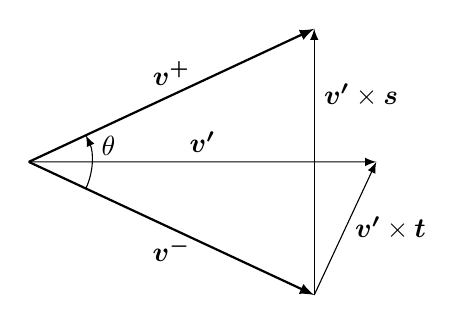
\begin{tikzpicture}[
	scale=2,
	>=latex]

	\def\centerarc[#1](#2)(#3:#4:#5)% Syntax: [draw options] (center) (initial angle:final angle:radius)
		{\draw[#1] ($(#2)+({#5*cos(#3)},{#5*sin(#3)})$) arc (#3:#4:#5); }

	\def\startangle{-25}
	\def\midangle{0}
	\def\endangle{25}
	\def\radius{2.0}
	\pgfmathsetmacro{\vlen}{\radius*tan(\startangle)}%

	\coordinate (O) at (0,0);
	\coordinate (S) at (\startangle:\radius);
	\coordinate (E) at (\endangle:\radius);

%	\centerarc[dashed](O)(\startangle:\endangle:\radius);
	\centerarc[->](O)(\startangle:\endangle:0.2*\radius);

	\draw (O)+(0.4,0.1) node [right] {$\theta$};

	\draw [thick,->] (O) -- (E) node [midway, above] {$\V{v^+}$};
	\draw [thick,->] (O) -- (S) node [midway, below] {$\V{v^-}$};

	\path (S) +(\startangle-90:\vlen) coordinate (V1E);
%	\path (E) +(\endangle-90:\vlen) coordinate (V3E);

%	%\draw [->] (E) -- (V3E);
	\draw [->] (S) -- (V1E) node [midway, right] {$\V{v'} \times \V t$};
%
	\draw [->] (O) -- (V1E) node [midway, above] {$\V{v'}$};
	\draw [->] (S) -- (E) node [near end, right] {$\V{v'} \times \V s$};

%	\draw [fill=white] (O) circle (0.02);

\end{tikzpicture}
\caption{Velocity space rotation from $\v-$ to $\v+$}
\end{figure}
%
\paragraph{Add half electric impulse} We define $\V{v^-}$ as the velocity after 
half a electric impulse:
$$\v^- = \v_{t-\dt/2} + \frac{q \E}{m} \frac{\dt}{2}$$

\paragraph{Rotate for the magnetic field} The rotation is done in two steps, 
first the half rotation is computed, with an angle of $\theta/2$:
$$\v' = \v^- + \v^- \times \V t $$

Then the rotation is completed by symmetry, using the $\V s$ vector
$$ \V s = \frac{2 \V t}{1 + \V t^2} $$
as
$$ \V{v^+} = \V{v^-} + \V{v}' \times \V{s} $$

\section{Field solver}

Talk about MFT and the data layout.

\section{Data structures}

The simulator is designed for space domains of one or two dimensions. In order 
to parallelize the computation of each step, the space domain is distributed in 
blocks. First the space domain is split in one specific dimension into MPI 
blocks, which will be distributed among each compute node. Communications will 
be needed to share information between MPI blocks.

The second hierarchy splits MPI blocks into task blocks, which can run in 
parallel inside a compute node. Communications are not needed, as we can use 
shared memory in the same compute node.

Inside each task block, we have a small portion of the space domain: the grid 
points of the fields and the particles inside the physical space of the block.  
Additionally, ghost points are placed at the boundaries of the positive 
neighbours in each dimension of the problem.

% TODO; Write about ghost points, and why they are needed

\begin{figure}[h]
	\centering
	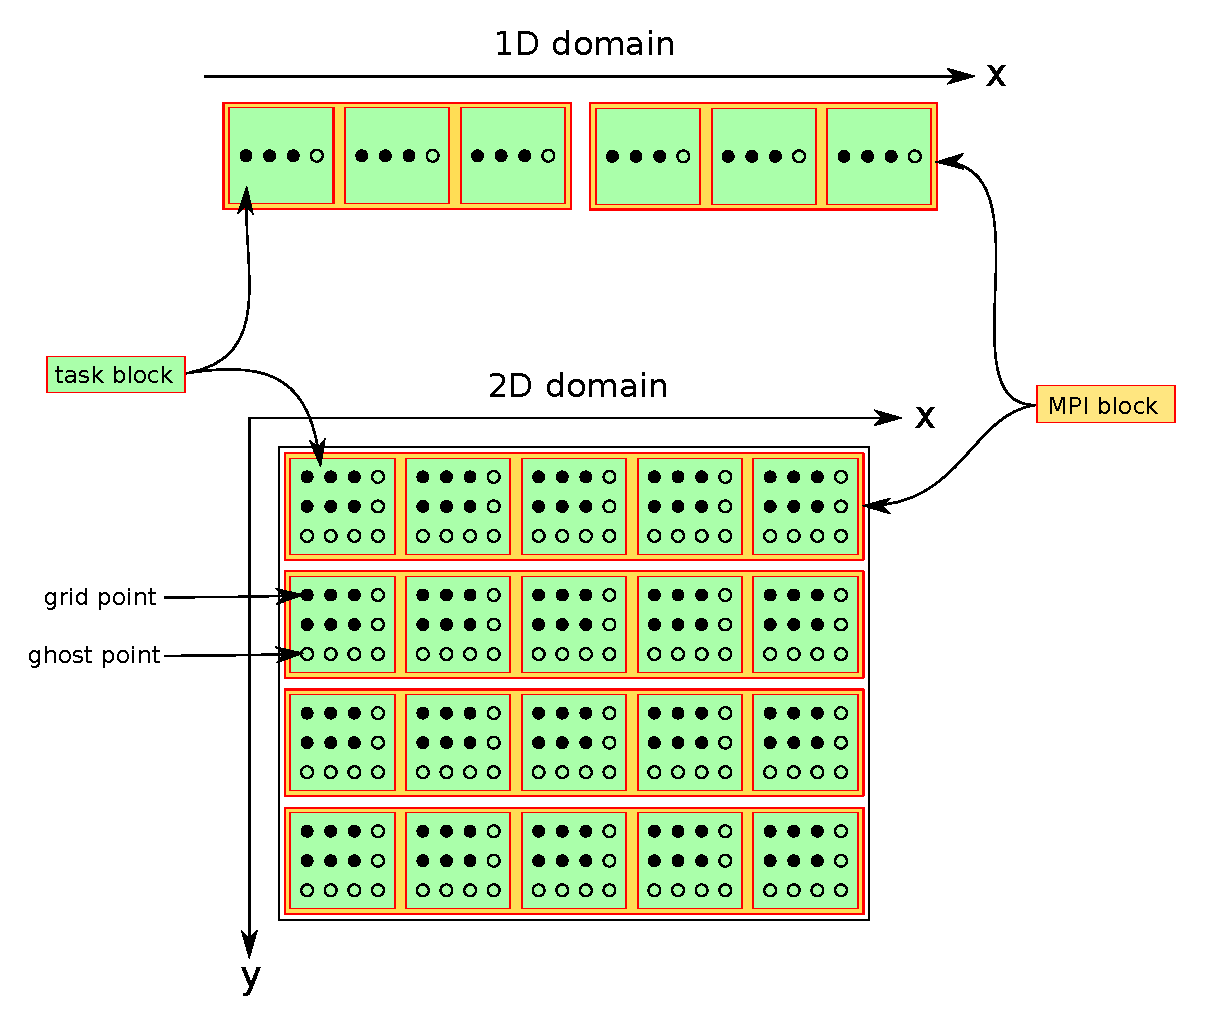
\includegraphics[width=\linewidth]{domain-blocks.pdf}
	\caption{Domain blocks}
	\label{fig:domain-blocks}
\end{figure}

A summary of the data layout can be seen in the figure \ref{fig:domain-blocks}, 
where the physical placement of each block corresponds to the physical position 
of the grid points. The 1D domain has 2 MPI blocks with 3 task blocks each, and 
3 grid points per block with 1 ghost point. In total, the space is discretized 
	in 18 grid points, which require 24 with the ghost points.

Similarly, for 2D the number of ghost points increase, as the frontier now has 2 
dimensions, leading to blocks with 6 grid points and 6 ghost points. The whole 
domain is discretized in 120 grid points, a total of 240 with ghost points.



\chapter{Analysis}

%\section{Analyze time distribution}

In order to reduce the amount of CPU time involved in each step of the 
simulation, the best strategy is to reduce the time spent in the most time 
consuming part.

The CPU time involved in each part of the simulation may depend on various 
factors, such as the number of grid points, the number of particles or the 
boundary conditions. As an example, consider a simulation with a large number of 
grid points, with few particles---the computation of the electric field 
(\texttt{field\_E}) will dominate the simulation time, as shown in the figure 
\ref{fig:cm-big-grid}. In a case of a large number of particles and a smaller 
grid, the particle interpolation (\texttt{particle\_E}) dominates the whole 
execution as seen in the figure \ref{fig:cm-lots-particles}.

\begin{figure}[h]
	\centering
	\subfloat[1024 particles, 512x512 grid points]{
		\includegraphics[width=\linewidth]{callmap-grid512x512-n1024.png}
		\label{fig:cm-big-grid}
	}
	\\
	\subfloat[10240 particles, 64x64 grid points]{
		\includegraphics[width=\linewidth]{callmap-grid64x64-n10240.png}
		\label{fig:cm-lots-particles}
	}
	\caption{Comparison of the time spent in each function at two different 
	simulations.}
\end{figure}

In order to optimize the general use case, different inputs will be tested and 
the main simulation steps will be characterized. Furthermore, different 
algorithms or methods may be used to improve the speed. As an example, the LU 
algorithm is compared with the spectral method MFT.

\section{Analysis with varying inputs}



%
%\chapter{Results}
%
%\chapter{Conclusions}

%\bibliographystyle{siam}
%\bibliography{bib}

\end{document}
